% Copyright 2004 by Till Tantau <tantau@users.sourceforge.net>.
%
% In principle, this file can be redistributed and/or modified under
% the terms of the GNU Public License, version 2.
%
% However, this file is supposed to be a template to be modified
% for your own needs. For this reason, if you use this file as a
% template and not specifically distribute it as part of a another
% package/program, I grant the extra permission to freely copy and
% modify this file as you see fit and even to delete this copyright
% notice. 

\documentclass{beamer}

% There are many different themes available for Beamer. A comprehensive
% list with examples is given here:
% http://deic.uab.es/~iblanes/beamer_gallery/index_by_theme.html
% You can uncomment the themes below if you would like to use a different
% one:
% \usetheme{AnnArbor}
% \usetheme{Antibes}
% \usetheme{Bergen}
% \usetheme{Berkeley}
% \usetheme{Berlin}
% \usetheme{Boadilla}
% \usetheme{boxes}
% \usetheme{CambridgeUS}
% \usetheme{Copenhagen}
% \usetheme{Darmstadt}
%\usetheme{default}
% \usetheme{Frankfurt}
% \usetheme{Goettingen}
\usetheme{Hannover}
% \usetheme{Ilmenau}
% \usetheme{JuanLesPins}
% \usetheme{Luebeck}
% \usetheme{Madrid}
% \usetheme{Malmoe}
% \usetheme{Marburg}
% \usetheme{Montpellier}
% \usetheme{PaloAlto}*
% \usetheme{Pittsburgh}
% \usetheme{Rochester}
% \usetheme{Singapore}
% \usetheme{Szeged}
% \usetheme{Warsaw}
\graphicspath{ {images/} }
\setbeamertemplate{footline}[frame number]  
\title{Parallel Automata Processing Review}

% A subtitle is optional and this may be deleted
% \subtitle{Emerging Architectures}

\author{Jose Chavez\inst{.}}
% - Give the names in the same order as the appear in the paper.
% - Use the \inst{?} command only if the authors have different
%   affiliation.

\institute[University of Engeeniering and Technology] % (optional, but mostly needed)
{
  \inst{.}%
  Department of Computer Science\\
  University of Engeeniering and Technology
  }
% - Use the \inst command only if there are several affiliations.
% - Keep it simple, no one is interested in your street address.

\date{Operating Systems, 2019}
% - Either use conference name or its abbreviation.
% - Not really informative to the audience, more for people (including
%   yourself) who are reading the slides online

\subject{Theoretical Computer Science}
% This is only inserted into the PDF information catalog. Can be left
% out. 

% If you have a file called "university-logo-filename.xxx", where xxx
% is a graphic format that can be processed by latex or pdflatex,
% resp., then you can add a logo as follows:

% \pgfdeclareimage[height=0.5cm]{university-logo}{university-logo-filename}
% \logo{\pgfuseimage{university-logo}}

% Delete this, if you do not want the table of contents to pop up at
% the beginning of each subsection:
% \AtBeginSubsection[]
% {
%   \begin{frame}<beamer>{Outline}
%     \tableofcontents[currentsection,currentsubsection]
%   \end{frame}
% }

% Let's get started
\begin{document}
\begin{frame}
  \titlepage
\end{frame}

\begin{frame}{Outline}
  \tableofcontents
  % You might wish to add the option [pausesections]
\end{frame}

\section{Main Concepts}

\subsection{Finite State Machines (FSM)}

\begin{frame}[allowframebreaks]{Finite State Machines}{FSM definition}
\begin{itemize}
    \item Formally described by a quintuple $\langle$ Q, $\sum$, $\delta$ , $q_0$ , F$\rangle$.
    
        \item Q is a set of states.
        \item $\sum$  is the input symbol alphabet.
        \item $\delta(Q,\alpha)$ is the transition function
        \item $q_0$ is the set of start states.
        \item F is the set of reporting or accepting states.  
            
     
            \item   \begin{figure}[!h]
                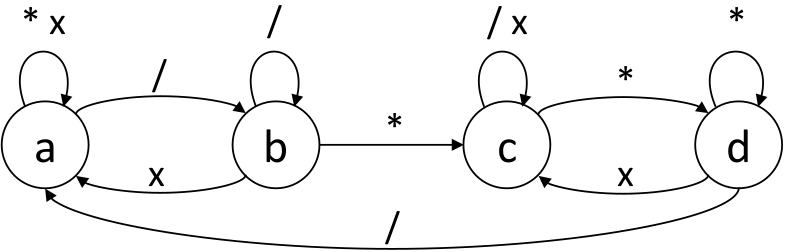
\includegraphics[width=0.7\textwidth]{fsmestado.png}
                \caption{State representation(NFA)[2]}
                \end{figure}
        \item   \begin{figure}[!h]
            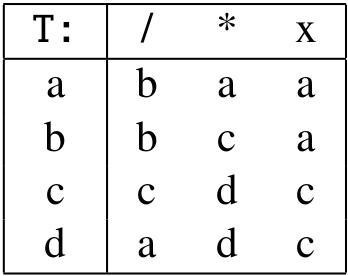
\includegraphics[width=0.35\textwidth]{fsmmatrix.png}
            \caption{Transition Table representation[2]}
            \end{figure}
    
                
    \end{itemize}
    
\end{frame}

  \subsection{The Micron Automata Processor  (AP)}

  % You can reveal the parts of a slide one at a time
  % with the \pause command:
  \begin{frame}[allowframebreaks]{The Micron Automata Processor (AP)}
    \begin{itemize}
    \item {
      \begin{figure}[!h]
          
\includegraphics[width=0.3\linewidth]{index.jpeg}
          \centering
      \end{figure}
    }
    \item {   
      \begin{figure}[!h]
          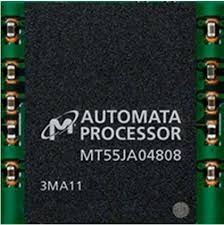
\includegraphics[width=0.5\linewidth]{automata.jpeg}
      \end{figure}
    }
    
          \item {"Micron’s 48-chip evaluation board scales this bandwidth to a ridiculous 38TB/s, which enables Automata to solve problems that traditional processors cannot." -\textit{Micron}
          \begin{figure}[!h]
          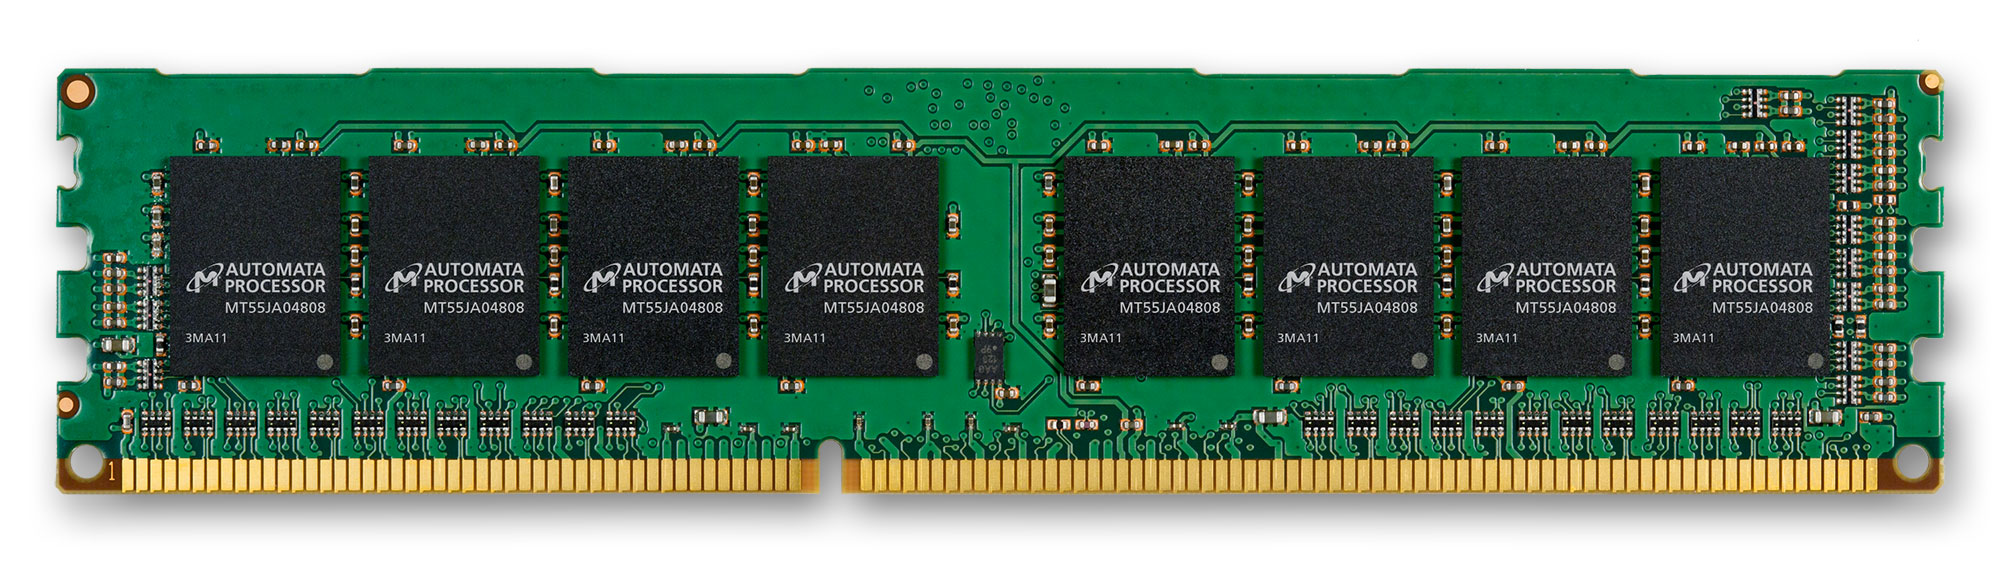
\includegraphics[width=1\linewidth]{high_res_automata_dimm.jpg}
              
          \end{figure}}
      \end{itemize}
      
      
  \end{frame}
  \section{Problems}

  \begin{frame}{Problems}
  \begin{itemize}
      \item These embarrassingly sequential
      applications (FSM) with irregular memory access patterns perform poorly
      on conventional von-Neumann architectures.
      \item FSM computation, especially Non-Determinstic Finite Automata
      (NFA) computation is inherently hard to speedup.
      \item Modern multi-core processors are limited by the number of transitions they can do
      per thread in a given cycle, limiting the number of patterns they can
      identify.
      
  \end{itemize}
  \end{frame}

  % Placing a * after \section means it will not show in the
  % outline or table of contents.
  \section{Solution}
  \subsection{Theorical Solution}
  \begin{frame}[allowframebreaks]{Theorical Solution}
      Partitioning the input string into segments and processing these segments concurrently.\\
      The problem with this approach is that starting states
  for each segment are unknown except the first segment. 
  \begin{enumerate}
    \item Represent the NFA with a compact equal form, that is the  AutomataNetwork  Markup  Language (ANML) NFA
    \item We look up for destination states by the transition table and we convert them into active states for the next step.
    \item We stablish the routing matrix an use it to store the transitions and the function.
    \item Determine the set of states that are active in a particular cycle.
  \end{enumerate}        
    
  \end{frame}

  \subsection{Parellel FSM}

  \begin{frame}[allowframebreaks]{Parellel FSM}
    \begin{figure}[!h]
    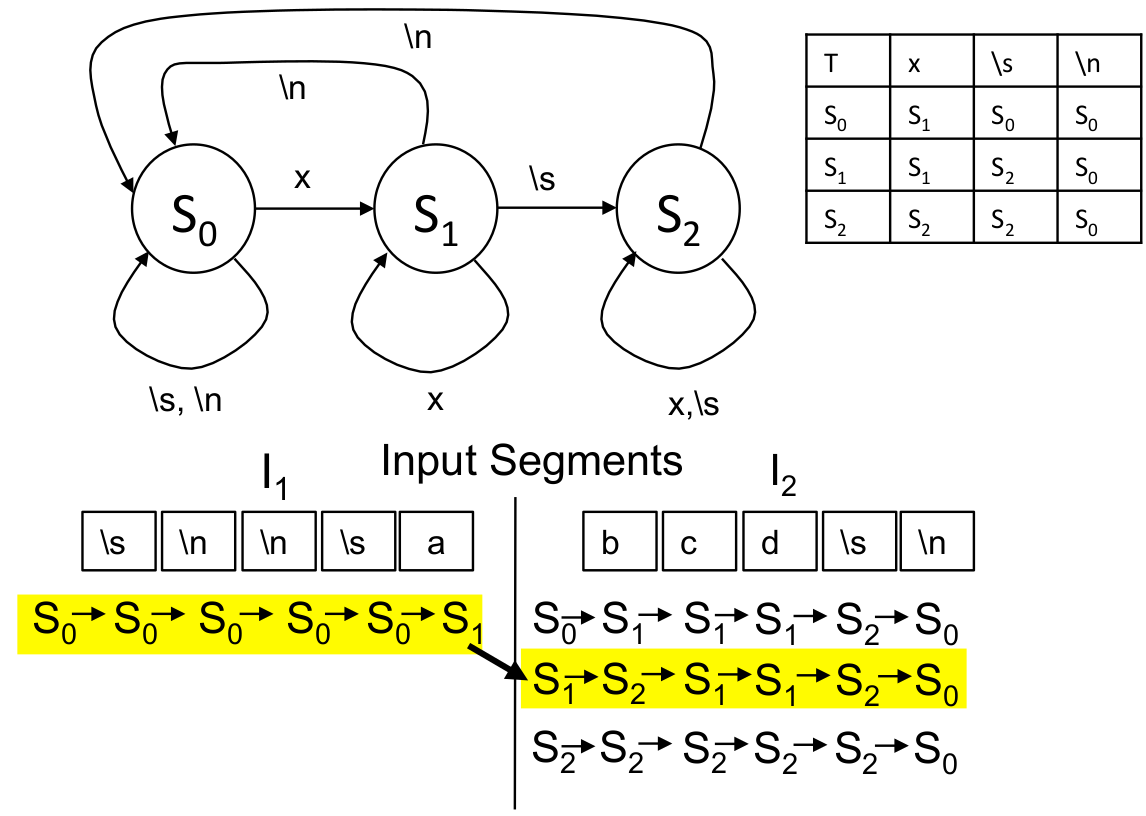
\includegraphics[width=0.5\linewidth]{f3.png} 
    \caption{A FSM example with enumeration[1]}   
    \end{figure}
    \begin{block}{Base Enumerative Technique}
      Stores a list of states at each step, insted of a single state.
    \end{block}
  \end{frame}

  \section{Overall Speedup}
  \begin{frame}[allowframebreaks]{Overall Speedup}
    With these implementations we reach a \textbf{theoretical 2$x$(number of partitions)} over sequential baseline.\\
    And in a \textbf{experimental} result we reached a significant speedup of \textbf{25.5$x$} on average compared again with sequential execution.
  \end{frame}

  % All of the following is optional and typically not needed. 
  \appendix
  \section<presentation>*{\appendixname}
  \subsection<presentation>*{Reference}

  \begin{frame}[allowframebreaks]
    \frametitle<presentation>{Reference}
      
    \begin{thebibliography}{10}
      
    % \beamertemplatebookbibitems
    % % Start with overview books.

    \bibitem{1}
    Aron Subramaniyan
      \newblock {\em Parallel Automata Processor}.
      \newblock ISCA '17 June.
  
      
    % \beamertemplatearticlebibitems
    % % Followed by interesting articles. Keep the list short. 

    \bibitem{2}
      Todd Mytkowicz.
      \newblock Data-Parallel Finite-State Machines
      \newblock {\em ASPLOS'14 March.}
    \end{thebibliography}
  \end{frame}

\end{document}


